\appendix
\raggedbottom

\section{Reservoir model, dissipator construction, and shared methods}
\label{app:shared}
\label{sec:methods}

This appendix gives the shared definitions and numerical conventions, then
the additional controls and interpretation behind each analysis.

\subsection{Data and code availability}
\label{app:reproducibility}

All code, data, and analysis workflows for this work, together with the
manuscript source and figure inputs, are available at
\url{https://github.com/eybmits/qrc-dissipation-engineering}. The repository
documents the full protocol, including random seeds, Hamiltonian and input
definitions, data splits, parameter grids, solver and optimization settings,
and numerical tolerances. It also contains the calibration records,
convergence checks, and per-run outputs behind each reported number, so every
result in the paper can be inspected and reproduced.

\subsection{Collective process, pairing, and readout}
\label{app:collective-process}

The principal collective process uses one fixed vector in the main,
finite-size, Hamiltonian, activity-matched, and gap-matched comparisons:
\[
  c_i=1\quad(i=1,\ldots,N),\qquad
  \boldsymbol c=(1,\ldots,1),\qquad
  L_{\mathrm c}=\sqrt{\gamma}\sum_{i=1}^{N}\sigma_i^- .
\]
Thus the coefficients are real, have equal phase, and satisfy
\(\sum_i|c_i|^2=N\).  Only the separately identified profile-by-family check
fits a nonuniform collective profile.  The common target is the unit-rate
local value \(\mathcal B=N2^{N-1}\), giving \(\mathcal B=80\) at \(N=5\).
The finite-size study rematches this target separately at every \(N\).

The jump-family comparison uses independently drawn complete-graph couplings
\(J_{ij}\sim U[-1,1]\).  Unless a control explicitly changes an operating
point, \(h=\Delta t=0.5\), the reservoir starts in
\(\lvert0\cdots0\rangle\), and the STM and NARMA-10 sequences contain 200
washout, 600 training, and 400 test inputs. The task-specific parity and
MG-150 protocols are stated below. Comparisons are paired: for a given seed,
all dissipative designs see the same Hamiltonian, input sequence, targets,
and data split.  Variation across seeds therefore reflects both a new
reservoir and a new input sequence.

At \(N=5\), the readout contains the expectations of all one-qubit Pauli
operators and all same-axis two-qubit Pauli products.  These 45 measured
features, together with a bias, feed a linear classical readout.  The internal
quantum dynamics are not trained.  Continuous-input evolution is computed by
sparse matrix exponentiation.  The dense-grid approximation used only for
the bounded local-profile search is described in
Appendix~\ref{app:experiment2}.

\subsection{Tasks and what they probe}

Short-term memory (STM) asks whether a past input can be reconstructed from
the present reservoir state.  We sum the squared-correlation capacities for
delays \(1,\ldots,20\).  Larger values mean that more of the recent input
history remains linearly accessible.

NARMA-10 adds nonlinear temporal processing.  Its target obeys
\[
\begin{aligned}
y_k={}&0.3y_{k-1}+0.05y_{k-1}\sum_{j=1}^{10}y_{k-j}\\
&+1.5\tilde s_{k-10}\tilde s_{k-1}+0.1,
\qquad \tilde s=0.2s ,
\end{aligned}
\]
and is scored by normalized mean-squared error (NMSE), so smaller is better.
Parity uses binary input windows of length \(1,\ldots,7\) and 15 virtual
nodes per input interval.  It has separate 500/250/400
train/validation/test streams after 100 washout inputs.  Validation selects
the readout regularization before a train-plus-validation refit.

The forecasting target obeys the Mackey--Glass equation
\[
\dot x(t)=\frac{0.2x(t-17)}{1+x(t-17)^{10}}-0.1x(t).
\]
It is integrated by Euler steps of length one from the seeded delay history
\(x_t=1.2+0.01\xi_t\), with
\(\xi_t\overset{\mathrm{iid}}{\sim}\mathcal N(0,1)\). Every third Euler
iterate is retained, and the first 500 retained samples are discarded. After a
200-sample washout and 600-sample teacher-forced training prefix, the readout
is closed for 150 steps.  The affine scale
is fixed by the washout-plus-training prefix.  Only closed-loop predictions
fed back to the reservoir are clipped to \([0,1]\), while the held-out target
remains unclipped.

For Table~\ref{tab:map}, each continuously driven design and the external
reset-FN baseline uses 32 reservoirs for STM and NARMA-10, 16 for parity, and
64 for MG-150. The no-dissipation diagnostic uses 30, 30, 32, and 32
reservoirs, respectively.

\begin{table}[!t]
\centering
\caption{\textbf{Absolute scores for the fixed-\(\mathcal B\),
common-protocol comparison.}
Entries are mean \(\pm\) standard error. Arrows give the favorable direction,
and bold marks the best mean. Row groups distinguish external or diagnostic
comparisons, fixed-profile jump-family models, and a profile-only variation
within local relaxation. Task definitions and sample sizes are stated
immediately above.}
\label{tab:map}
\scriptsize
\setlength{\tabcolsep}{4pt}
\renewcommand{\arraystretch}{0.96}
\resizebox{\linewidth}{!}{%
\begin{tabular}{@{}lcccc@{}}
\toprule
model & STM \(\uparrow\) & NARMA-10 \(\downarrow\)
 & parity \(\uparrow\) & MG-150 \(\downarrow\)\\
\midrule
\multicolumn{5}{@{}l}{\emph{External and diagnostic comparisons}}\\
no dissipation
 & \(0.047\pm0.004\) & \(1.308\pm0.036\)
 & \(0.016\pm0.001\) & \(0.0697\pm0.0016\)\\
reset-encoded FN~\cite{Fujii2017}
 & \(10.106\pm0.260\) & \(0.367\pm0.012\)
 & \(2.295\pm0.125\) & \(0.115\pm0.008\)\\
\addlinespace[2pt]
\multicolumn{5}{@{}l}{\emph{Fixed-profile jump-family models}}\\
uniform local relaxation~\cite{Sannia2024}
 & \(8.634\pm0.069\) & \(0.315\pm0.008\)
 & \(4.822\pm0.038\) & \(0.0369\pm0.0029\)\\
collective relaxation
 & \(\mathbf{12.206\pm0.101}\) & \(\mathbf{0.229\pm0.006}\)
 & \(3.782\pm0.028\) & \(0.0969\pm0.0091\)\\
pair loss
 & \(9.203\pm0.082\) & \(0.289\pm0.007\)
 & \(4.752\pm0.037\) & \(0.0387\pm0.0035\)\\
local gain/loss
 & \(8.307\pm0.058\) & \(0.337\pm0.008\)
 & \(4.852\pm0.044\) & \(0.0462\pm0.0038\)\\
exchange-assisted relaxation
 & \(7.413\pm0.045\) & \(0.441\pm0.009\)
 & \(\mathbf{5.083\pm0.049}\) & \(0.0518\pm0.0038\)\\
dephasing
 & \(0.000\pm0.000\) & \(1.020\pm0.006\)
 & \(0.000\pm0.000\) & \(0.0599\pm0.0004\)\\
\addlinespace[2pt]
\multicolumn{5}{@{}l}{\emph{Profile-only variation within local relaxation}}\\
unequal local relaxation
 & \(9.845\pm0.119\) & \(0.266\pm0.007\)
 & \(4.366\pm0.071\) & \(\mathbf{0.0349\pm0.0028}\)\\
\bottomrule
\end{tabular}%
}
\end{table}

\subsection{Constructing and normalizing dissipative processes}

Table~\ref{tab:designs} gives the physical action of the six process families
and the unequal-rate variant.  Unequal local rates are drawn log-uniformly
from \([0.1,10]\) and rescaled to unit mean.  The collective coefficients are
the fixed equal-phase choice \(c_i=1\) stated in
Appendix~\ref{app:collective-process}.  Pair loss contains every \(i<j\).
Exchange-assisted relaxation combines local lowering with ordered,
excitation-conserving exchange jumps, assigning 40\% of \(\mathcal B\) to
the former and 60\% to the latter.  The local gain/loss process uses
downward/upward rates \(1/0.3\) before the common rescaling.  After
construction, one scalar rescales every completed design to the same
\(\mathcal B=\sum_k\Tr(L_k^\dagger L_k)\) as unit-rate uniform local
relaxation.

Section~\ref{sec:model} defines the fixed operator basis and Kossakowski matrix
used to compare generators independently of jump-list remixing. For the
one-body lowering families, write
\[
L_k=\sum_i A_{ki}\sigma_i^-,
\qquad
\Gamma=A^\dagger A\succeq0 .
\]
Then
\[
\mathcal B=2^{N-1}\Tr\Gamma .
\]
Thus fixed \(\mathcal B\) fixes \(\Tr\Gamma\). Uniform local relaxation has
rank \(N\), whereas the equal-phase collective channel has rank one. Kernel
directions are Kossakowski coupling directions, not decay modes of the full
Liouvillian; Hamiltonian mixing can provide indirect relaxation. The identity
above applies only to the one-body lowering block. Across unlike operator
sectors, fixed \(\mathcal B\) remains a structural control rather than an
equivalence of spectra, flows, or implementation cost.

\subsection{Statistical reporting}

All primary effects are computed as paired, instance-level differences and
oriented so that positive means improvement.  Unless stated otherwise, we
report the mean difference, a two-sided 95\% Student-\(t\) interval, and the
paired win count. For the non-reference cell comparisons, paired sign-flip
tests are corrected over the comparison family
with the Holm procedure~\cite{Holm1979}. Finite-size intervals use paired
bootstrap resampling. The profile and finite-sampling experiments use
simultaneous intervals because many related contrasts are examined together.

\FloatBarrier
\section{Jump-family computation and local--collective controls}
\label{app:experiment1}

The jump-family analysis asks whether changing the jump family changes
computation when the Hamiltonian, input, operating point, readout, and
\(\mathcal B\) are held fixed.  The broad map establishes the task dependence
of that jump-family choice.  The subsequent checks focus on the principal
collective-versus-local memory contrast.

\subsection{Fixed-\texorpdfstring{\(\mathcal B\)}{B} jump-family task map}

Figure~\ref{fig:map} and Table~\ref{tab:map} report the absolute
fixed-\(\mathcal B\) scores; Figure~\ref{fig:rank-map} gives the complementary
rank view.

A validation-selected readout control reuses the same STM and NARMA-10
trajectories but divides the 600 fitting rows into 450 training and 150
validation rows.  Each design and instance selects ordinary least squares or
a ridge value before refitting on all 600 rows.  The ordering is unchanged:
the collective design remains best on both tasks.  Thus the main ranking is
not an artifact of imposing one readout penalty on every process.

\begin{figure}[!t]
\centering
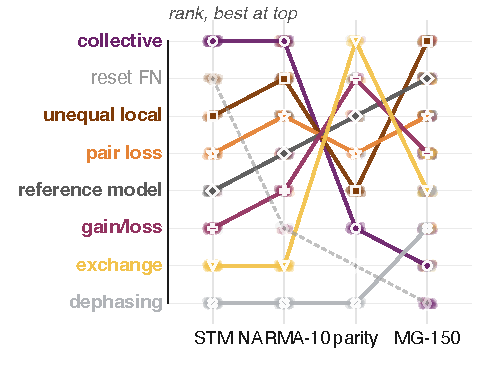
\includegraphics{figures/fig_map.pdf}
\caption{\textbf{Task-wise rankings confirm specialization rather than a
universal winner among the tested continuously driven designs.}
Ranks at \(N=5\) are induced by the absolute means in
Table~\ref{tab:map}; rank 1 is best within each task. Uniform local is the
reference. Colors follow the manuscript-wide dissipator palette; lines connect
identical designs only as visual guides. Dashed reset-based FN is an external,
unpaired baseline. Faint points rank the paired continuously driven seeds
against the fixed reset-FN mean; no seed points are assigned to that baseline.}
\label{fig:rank-map}
\end{figure}

\subsection{Robustness to the coherent dynamics}

The principal contrast was repeated in four paired \(N=5\) spin-Hamiltonian
ensembles: the primary \(XX+Z\) model with an \(X\) drive, a \(ZZ+X\) model
with a \(Z\) drive, an \(XY+Z\) model with an \(X\) drive, and an \(XX\) ring
with an \(X\) drive. The encoding and Pauli readout remain fixed.

\subsection{Replication under reset-based input encoding}
\label{app:reset-architecture}

To test whether the local--collective ordering depends on continuous-drive
encoding, we repeat the comparison in a reset-encoded reservoir. At input
step \(t\), qubit zero is replaced by
\[
 \rho_t^{+}
 = \lvert\psi(s_t)\rangle\!\langle\psi(s_t)\rvert_0
   \otimes \Tr_0(\rho_t),
 \qquad
 \lvert\psi(s)\rangle
 = \sqrt{1-s}\lvert0\rangle+\sqrt{s}\lvert1\rangle ,
\]
after which the autonomous \(XX+Z\) Hamiltonian evolves together with either
uniform local relaxation or the equal-phase collective channel. This changes
the input architecture: the reset is non-unitary and the input-dependent
transverse drive is absent during the evolution interval.

The strict comparison otherwise retains the principal \(N=5\) construction:
complete-graph couplings independently drawn from \(U[-1,1]\),
\(h=\Delta t=0.5\), \(\gamma=1\), \(\mathcal B=80\), i.i.d. inputs
\(s_t\sim U[0,1]\), the 45 Pauli features and bias, ridge \(10^{-8}\), STM
delays \(1,\ldots,20\), the same NARMA-10 target, and 600 training and 400
untouched test inputs. Within each of 16 fresh pairs, the local and collective
reservoirs share the Hamiltonian, input sequence, target, and data split. We
use an 800-input washout because
collective reset dynamics converge more slowly than their local counterpart.
Table~\ref{tab:reset-architecture} reports the strict task endpoints, and
Figure~\ref{fig:reset-architecture} shows their paired effects and
lag-resolved STM profile.

\begin{table}[H]
\centering
\caption{\textbf{Strict reset-encoded replication.} The effect is
collective-minus-local for STM and local-minus-collective for NARMA-10, so
positive values are favorable in both rows. Intervals are paired \(95\%\)
confidence intervals.}
\label{tab:reset-architecture}
\footnotesize
\setlength{\tabcolsep}{3.5pt}
\renewcommand{\arraystretch}{1.08}
\begin{tabular}{@{}lcccc@{}}
\toprule
task & local & collective & favorable effect & wins\\
\midrule
STM capacity
 & \(4.595912\) & \(6.369394\)
 & \(1.773\,[1.312,2.235]\) & \(16/16\)\\
NARMA-10 NMSE
 & \(0.672973\) & \(0.490933\)
 & \(0.182\,[0.144,0.220]\) & \(16/16\)\\
\bottomrule
\end{tabular}
\end{table}

\begin{figure}[H]
\centering
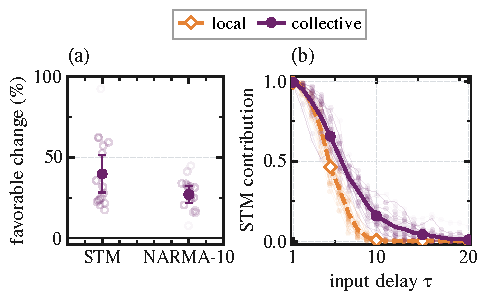
\includegraphics{figures/fig_reset_architecture.pdf}
\caption{\textbf{Replication under reset-based input encoding.}
\emph{(a)} Favorable paired relative change with respect to local relaxation
for STM capacity and NARMA-10 NMSE across 16 fresh paired reservoirs; positive
percentages denote larger STM or lower NMSE. Points show seeds, and filled
markers with bars show paired means and pointwise \(95\%\) \(t\) intervals.
\emph{(b)} Lag-resolved STM capacities after the strict 800-input washout;
faint lines and points are seeds, and thick lines and bands show means and
pointwise \(95\%\) \(t\) intervals. The fixed-budget comparison uses
\(\gamma=1\) and \(\mathcal B=80\).}
\label{fig:reset-architecture}
\end{figure}

Repeating both tasks and both dissipative models from the ground, fully
excited, maximally mixed, and Haar-random pure states gives a maximum score
range below \(7\times10^{-7}\); the largest trace distance at the 800-input
washout is \(1.3\times10^{-14}\), at numerical precision. The strict ordering
therefore reflects retained input history rather than the tested starting
state. It establishes that the effect transfers across the two tested input
architectures, not universal architecture independence. Nor does this
comparison imply that dissipation outperforms a reset-only unitary reservoir;
it isolates how two matched environmental-coupling designs shape usable memory.

\subsection{Finite size and loss of the initial state}

The finite-size study uses 24 fresh paired lineages at every
\(N=4,\ldots,8\).  Nested principal submatrices of an \(N=8\) coupling draw
are rescaled by \(\sqrt{4/(N-1)}\), and the Frobenius reference is rematched
within each size.  The number of measured Pauli features, excluding the fitted
bias, grows as
\[
F(N)=3N+3\binom{N}{2}.
\]
The sweep is intended as a finite-size robustness test of the paired
local--collective ordering, not as an analysis of asymptotic memory,
mixing-time, or Liouvillian scaling. STM is summed over a fixed 20-delay
horizon and therefore satisfies \(C_{\mathrm{STM}}\leq 20\) for every \(N\),
whereas \(F(N)\) grows with \(N\). Consequently,
\[
  \frac{C_{\mathrm{STM}}}{F(N)}
  \leq \frac{20}{3N+3\binom{N}{2}}.
\]
Even perfect recall at all tested delays would therefore have a decreasing
STM-per-feature ceiling. This ratio is not a neutral scaling or
resource-efficiency metric under the present protocol. The grouped readout
still requires only the three global \(X\), \(Y\), and \(Z\) settings, while
the fitted linear readout has \(F(N)+1\) inputs after including the bias.
Figure~\ref{fig:collective-case}(b) shows the absolute scores across size.

Because collective coupling can leave some combinations only indirectly
damped, we separately tested whether the reported memory could be residual
dependence on the starting state.  For each process and size, eight fresh
lineages at \(N=4,5,6\) were driven by identical switched input sequences from
the ground, fully excited, maximally mixed, and a Haar-random pure state.
Every checkpoint stores the largest trace and Pauli-feature distances over
the six initial-state pairs. Local and pair processes converge rapidly. A
continuation follows all 48 local and pair lineages at
\(N=4,5,6\) to 1200 inputs; their worst trace distance over steps 1100--1200
is \(6.85\times10^{-15}\).
\Needspace{4\baselineskip}
For collective relaxation at the principal \(N=5\)
setting, the worst trace distance falls from \(4.78\times10^{-4}\) after 200
inputs to \(1.32\times10^{-11}\) after 800. A separate continuation
follows all eight lineages to 1200 inputs and reaches
\(4.42\times10^{-15}\), below its declared \(10^{-14}\) gate. The slowly
forgetting collective \(N=4\) boundary case is excluded from
initialization-independent claims.

A stricter STM check uses ten principal-pair lineages, three distant initial
states, and washouts of 50, 200, and 800 inputs. A separate continuous-drive
NARMA-10 check uses all 32 principal pairs. For its W800 condition, a frozen
600-input prefix is placed before the unchanged canonical 1200-input sequence;
the final 200 washout inputs and the 600 training and 400 test rows are thus
identical to W200. Local and collective reservoirs share every input, target,
split, Hamiltonian, and readout choice within a pair. Ground-state scoring uses
all 32 pairs, and the first eight repeat both washouts from the ground, fully
excited, maximally mixed, and Haar-random states. The W200 scores must reproduce
the sealed principal values before the W800 aggregate is accepted. At W800,
local and collective NMSE are \(0.315\) and \(0.230\), respectively; the
local-minus-collective difference is \(0.0851\,[0.0716,0.0986]\), favorable in
all 32 pairs. Its change from W200 is
\(-0.00007\,[-0.00057,0.00043]\). The largest four-state collective score spread
at W800 is \(2.18\times10^{-5}\), below the smallest paired ground-state
improvement, \(0.0148\). The archive records every checkpoint and the
serialization-only amendment made before any non-audit score was generated.

\subsection{Matched expected jump activity}
\label{app:activity-control}

The fixed-\(\mathcal B\) comparison deliberately allows the realized jump
activity to differ.  To test whether this alone explains the memory result,
we calibrate the two processes using the time-averaged expectation
\[
\mathcal J=\frac{1}{T\Delta t}\sum_{t=1}^{T}\int_0^{\Delta t}
\sum_k\Tr\!\left[L_k^\dagger L_k\rho_t(\tau)\right]\,\mathrm d\tau .
\]
Local and collective rates are fitted separately to
\(\mathcal J_\star=0.5075\) on a shared, unlabeled input stream that is
independent of every task stream.  After 100 washout inputs, activity is
averaged over 150 intervals.  All 16 calibrations for eight fresh reservoir
pairs pass the predeclared 1.5\% tolerance before task scoring.

\subsection{Matched midpoint Liouvillian gap}
\label{app:gap-control}

A second control asks whether the result is only a consequence of the slowest
relaxation time at a representative constant input.  For each of 24 fresh
\(N=5\) Hamiltonians, the local rate is calibrated to the collective
Liouvillian gap at \(s=0.5\) before task inputs are generated.  All
calibrations satisfy the 0.5\% relative-error gate.

\subsection{Independent operating-point selection}
\label{app:selection-control}
\label{app:selection-ablation}

The third control lets local and collective relaxation select their own
operating points without using test data.  The bounded search varies the drive,
input duration, dissipative strength, and readout penalty over predeclared
grids.  A two-reservoir prescreen
advances eight settings per jump family.
Twelve disjoint reservoirs then select one setting and readout penalty per
process.  The final 24 reservoirs are opened only after these choices are
written.  The collective strength choice is additionally bracketed on the
selection set before the final test.

\begin{figure}[H]
\centering
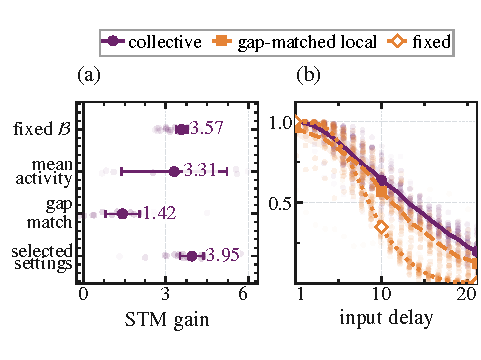
\includegraphics{figures/fig_scalar_controls.pdf}
\caption{\textbf{Targeted scalar controls preserve the local--collective
memory contrast.}
\emph{(a)} Collective-minus-reference STM effects for the fixed-\(\mathcal B\),
activity-matched, gap-matched, and independently selected protocols.
\emph{(b)} Lag-resolved STM at fixed \(\mathcal B\) and after matching the local
rate to the collective midpoint Liouvillian gap. Faint points show paired
seeds; bars and bands show the declared \(95\%\) intervals.}
\label{fig:scalar-controls}
\end{figure}

\subsection{Validation-selected scalar-strength sensitivity}
\label{app:strength-sensitivity}

The fixed-\(\mathcal B\) family map is a controlled jump-family slice rather
than a globally optimized ranking. In a complementary post hoc STM sensitivity
analysis, scalar strength is selected separately for six non-dephasing process
designs by leave-one-reservoir-out validation. All designs use the base
multiplier grid \(\{0.05,0.1,0.25,0.5,1,2,4\}\); uniform local and collective
relaxation also include \(8\) and \(16\), which bracket the collective optimum
at \(8\). The selected multipliers are \(8\) for collective, \(0.1\) for local
gain/loss and exchange-assisted relaxation, and \(0.25\) for uniform local,
unequal local, and pair loss; every curve is bracketed. Collective relaxation
has the largest mean across the 20 held-out scores, and 50,000 selection-aware
bootstrap draws give Bonferroni-simultaneous 95\% percentile intervals
whose lower endpoints are positive for its advantage over every competitor.
This supports the principal STM lead across the tested strength grid, but it
does not constitute a fully disjoint, task-wise optimized family ranking or a
four-task Pareto analysis.

\FloatBarrier
\section{Rate-profile optimization and comparison}
\label{app:experiment2}
\label{app:profiles}

The rate-profile analysis keeps the jump family fixed and changes only how
local relaxation strength is distributed across sites.  It therefore tests
the second coordinate of environmental-coupling organization independently of the jump-family
comparison.

\subsection{Within-family profile sweep}

The profile sweep uses \(N=5\), mean local rate 1.5,
\((h,\Delta t)=(0.5,0.5)\), and a shorter protocol tailored to profile
optimization.  It uses 100 washout inputs, 100 optimization-training inputs,
150 validation inputs, and 200 test inputs.  All static profiles have the
same arithmetic mean.  We compare a uniform reference with a random unequal
profile and a static profile learned on validation data.  A fourth model uses
the input-adaptive profile
\(\gamma_i(s)=\operatorname{softplus}(a_i s+b_i)\).  The adaptive profile is
matched only in mean over the frozen input grid, so its instantaneous
Frobenius strength may vary.

Static and adaptive profiles are optimized from seeded starts with fixed
evaluation limits and stopping rules.

\subsection{Does profile learning act the same way in every family?}

A separate \(2\times2\) check crosses local versus collective relaxation with
uniform versus learned profiles. Figure~\ref{fig:profiles}(b) displays the 24
paired trajectories and their mean changes.  Every candidate is normalized to
the same \(\mathcal B\), and exact continuous-input evolution replaces the dense
approximation.  For local relaxation, learning redistributes diagonal
sitewise rates.  For collective relaxation, it changes the coefficient vector
\(\boldsymbol c\) and thereby moves the supported one-dimensional
Kossakowski direction while preserving rank one.  The axes are therefore
operational and interacting design coordinates rather than a globally
orthogonal factorization. Inference uses simultaneous coverage over the eleven
declared contrasts.

\FloatBarrier
\section{Finite-sampling estimators and inference}
\label{app:experiment3}

The finite-sampling analysis asks whether the exact-expectation ordering remains
visible when Pauli features must be estimated from a finite number of
preparations.  It compares two estimators at the same nominal preparation
count, rather than treating shot noise as independent additive noise on every
feature.

\subsection{Two estimators at equal preparation count}

At \(N=5\), write \(N_{\mathrm{prep}}=45q\).  The independent estimator
spends \(q\) shots on each of the 45 observables.  The grouped estimator
instead spends \(15q\) shots in each global \(X\), \(Y\), and \(Z\) product
basis and reuses each measured bit string for all compatible one- and
two-qubit features.  Table~\ref{tab:sampling-estimators} emphasizes the
methodological difference without repeating the budget grid.

\begin{table}[H]
\centering
\caption{\textbf{Finite-sampling estimators at equal nominal preparation
count.} Grouping changes how measurement records are reused and therefore
preserves correlations between compatible Pauli estimates.}
\label{tab:sampling-estimators}
\footnotesize
\setlength{\tabcolsep}{6pt}
\renewcommand{\arraystretch}{1.12}
\begin{tabular}{@{}p{0.25\textwidth}p{0.33\textwidth}p{0.33\textwidth}@{}}
\toprule
 & independent observables & grouped Pauli settings\\
\midrule
recorded data
& one binomial estimate per feature
& full bit strings in \(X\), \(Y\), and \(Z\) bases\\
record reuse
& none across features
& one record informs all compatible features\\
covariance
& omitted by construction
& retained within each setting\\
modeled scope
& projection noise
& projection noise with grouping, without hardware noise\\
\bottomrule
\end{tabular}
\end{table}

\subsection{Training and simultaneous inference}

Six non-dephasing designs are evaluated on 20 paired reservoir and
measurement instances under both estimators.  Validation selects the readout
penalty from the predeclared grid before a
train-plus-validation refit.  We test \(q=64\times4^j\) for \(j=0,\ldots,6\),
so both estimators receive \(45q\) preparations per step.
Finite-budget intervals are simultaneous over every declared design-pair,
estimator, and budget contrast.  The exact-expectation endpoint is displayed
separately.

The curves in Figure~\ref{fig:sampling}(a,b) should therefore be read as a
resolution study. A design is distinguished from local relaxation only when
the simultaneous interval excludes zero, not merely when its mean is larger.
The model does not include acquisition latency, device drift, or gate and
readout errors.

\FloatBarrier
\section{Dynamical interpretation: support and limits}
\label{app:interpretation}

The following diagnostics test whether the observed response is consistent
with the shared-channel interpretation without claiming a unique microscopic
cause.

\subsection{Slow dynamics that remain visible to the readout}

For eight \(N=5\) local--collective lineages, the slowest right modes at five
constant inputs are projected onto the 45-Pauli readout span.  Collective
relaxation retains slower modes with larger overlap.  The paired differences
are \(0.338\,[0.239,0.436]\) in decay rate and
\(0.104\,[0.028,0.180]\) in readout-weighted retention. Because this omits
excitation weights and switched propagator products, it supports but does not
uniquely identify the shared-channel interpretation.

\subsection{Concentrated response under switched input}

Starting from synchronized trajectories, a complementary diagnostic applies
small input perturbations and follows the 45-feature response over 20 lags.
Collective relaxation concentrates this response in fewer observable
patterns than the matched local process.  Its effective rank is lower by
\(1.270\,[0.959,1.580]\), while the leading-pattern energy fraction is higher
by \(0.285\,[0.243,0.327]\).  The switched-input result supports the same
picture.  It is an empirical response kernel rather than a complete modal
decomposition.

\subsection{A gradual path from local to collective coupling}

To determine whether the endpoint contrast emerges along a continuous
coupling-organization path, we interpolate the dissipators at fixed Frobenius weight as
\(\D_\alpha=(1-\alpha)\D_{\mathrm{local}}
+\alpha\D_{\mathrm{collective}}\), with \(0\le\alpha\le1\).
Interior points are ranked on separate gap-only reservoirs before fresh task
streams are opened.  Increasing the collective component slows midpoint
relaxation and raises STM at \(N=4\) and \(5\).  The selected interior point
beats local relaxation in every fresh pair.  This links the endpoint result
to a continuous within-family deformation, not to a general selector for
unrelated processes.

\subsection{Why driven dephasing forgets uniformly}

The near-zero STM of the dephasing control admits a direct contraction
argument under the connectivity assumptions of the primary model.

\begin{proposition}[Uniform contraction of the driven dephasing model]
\label{prop:dephasing}
Let \(L_i=\sqrt{\gamma_i}Z_i\) with every \(\gamma_i>0\), let
\(\Phi_s=\exp(\Lind_s\Delta t)\) with \(\Delta t>0\), and suppose the nonzero
single-spin-flip matrix elements of \(H(s)\) connect the computational-basis
hypercube for every \(s\in[0,1]\). Then there is a \(\kappa<1\) such that
\[
\sup_{s\in[0,1]}
\left\|\Phi_s|_{\mathrm{Tr}=0}\right\|_{2\rightarrow2}\le\kappa .
\]
Here \(\|X\|_2=(\Tr X^\dagger X)^{1/2}\).  Hence
\(\|\rho_n-I/2^N\|_2\le\kappa^n\|\rho_0-I/2^N\|_2\) for any switched input
sequence and initial state.
\end{proposition}

\emph{Proof.}
For \(X_t=\exp(t\Lind_s)X\), the Hamiltonian commutator is skew-adjoint in the
Hilbert--Schmidt inner product, while the Hermitian-unitary jumps give
\(\frac{\mathrm d}{\mathrm dt}\|X_t\|_2^2
=-\sum_i\gamma_i\|[Z_i,X_t]\|_2^2\le0\).
Equality at \(\Delta t\) would make the norm constant, so every
\([Z_i,X_t]\) vanishes and \(X_t\) remains diagonal.  Its derivative can
remain diagonal only if \([H(s),X_t]=0\).  Hypercube connectivity then makes
\(X_t\) scalar.  Every nonzero traceless operator therefore contracts
strictly.  Attainment in finite dimension, continuity in \(s\), and
compactness of \([0,1]\) give one common \(\kappa<1\).\hfill\(\square\)

State differences are traceless, so the bound applies to every switched
sequence and all \(s\in[0,1]\).  It explains the dephasing zeros in
Table~\ref{tab:map} for the connected primary model, not arbitrary unital
dissipators.

\FloatBarrier
\section{Orientation within matched rank-one channels}
\label{app:phase-direction}

To vary the supported collective direction at fixed coarse channel invariants,
we use
\[
  c_i(f)=\exp\!\left[2\pi \mathrm{i}f(i-1)/5\right],\qquad
  f\in\{0,0.25,0.5,0.75,1\}.
\]
Here \(f=0\) is equal phase and \(f=1\) is orthogonal to the uniform direction.
Every condition has Kossakowski rank one, spectrum
\((5,0,0,0,0)\), unit diagonal, \(|c_i|=1\), magnitude IPR \(1/5\), and
\(\mathcal B=80\); four frozen phase-scrambled controls add zero-overlap
directions.

The confirmation uses 32 fresh paired reservoirs, excludes the pilot, and
shares Hamiltonian, input, target, split, and readout across all nine conditions
within each pair. After an 800-input washout, the unchanged protocol uses 600
training and 400 untouched test inputs, delays 1--20, 45 Pauli features, and
fixed ridge \(10^{-8}\). Four-state audits pass on the first eight lineages.

\begingroup
\setlength{\intextsep}{0pt}
\begin{figure}[H]
\centering
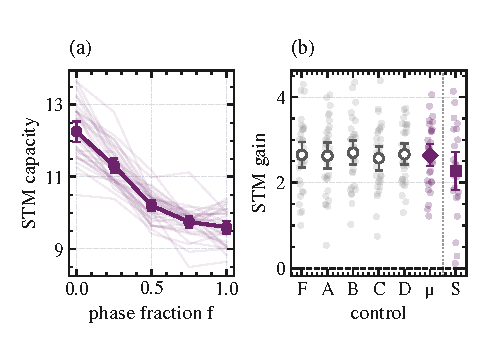
\includegraphics{figures/fig_phase_direction.pdf}
\caption{\textbf{Accessible memory depends on the matched rank-one direction.}
\emph{(a)} Prespecified \(N=5\) phase path. \emph{(b)} Equal-phase-minus-control
effects for five zero-overlap directions, their within-pair mean \(\mu\), and
the \(N=6\) sign-balanced replication S. Marks show pairs, means, and
\(95\%\) \(t\) intervals (32 and 24 pairs).}
\label{fig:phase-direction}
\end{figure}
\endgroup

Equal-phase STM is \(12.253\), versus \(9.604\) at the Fourier endpoint, a
paired difference of \(2.648\,[2.347,2.950]\) with \(32/32\) wins and
sign-flip \(p=1.0\times10^{-5}\). Against the within-pair mean of all five
zero-overlap directions, the gated effect is \(2.642\,[2.383,2.900]\), again
with \(32/32\) wins and \(p=1.0\times10^{-5}\). The ordered path and
validation-selected-ridge sensitivity agree.

\paragraph{Real sign-balanced replication at a second finite size.}
A separate 24-pair \(N=6\) endpoint replication compares
\(c_{+}=(1,1,1,1,1,1)\) with \(c_{\perp}=(1,1,1,-1,-1,-1)\), where
\(c_{+}^{\dagger}c_{\perp}=0\). At \(\mathcal B=192\), jump count, rank-one
spectrum \(\{6,0,0,0,0,0\}\), trace, diagonal weights, coefficient magnitudes,
processor, input, readout, data, and ridge rule remain fixed. All 24
ground/mixed-state audits and the first six four-state audits pass at W800.
Equal-phase STM is \(13.626\) versus \(11.354\), a paired gain of
\(2.271\,[1.826,2.717]\) with \(24/24\) wins and exact sign-test
\(p=1.19\times10^{-7}\); every delay-wise mean difference is positive. Thus
orientation affects accessible memory beyond these coarse matches, without
implying scaling, global optimality, or a unique mechanism.
